% Copyright 2004 by Till Tantau <tantau@users.sourceforge.net>.
%
% In principle, this file can be redistributed and/or modified under
% the terms of the GNU Public License, version 2.
%
% However, this file is supposed to be a template to be modified
% for your own needs. For this reason, if you use this file as a
% template and not specifically distribute it as part of a another
% package/program, I grant the extra permission to freely copy and
% modify this file as you see fit and even to delete this copyright
% notice. 

\documentclass[aspectratio=169]{beamer}
%\documentclass{beamer}

\setbeamersize{text margin left=5mm, text margin right=5mm}


\defbeamertemplate{headline}{my header}{%
\vskip1pt%
\makebox[0pt][l]{\,\insertshortauthor}%
\hspace*{\fill}\insertshorttitle/\insertshortsubtitle\hspace*{\fill}%
\llap{\insertpagenumber/\insertpresentationendpage\,}
}
\setbeamertemplate{headline}[my header]

\usepackage{soul}
\usepackage{tkz-euclide}
\usetikzlibrary{calc}
\usepackage[]{algorithm2e}
\usepackage{changepage}
\usepackage{amssymb}
\usepackage{xcolor}
\usepackage{mathtools}
\usepackage{tcolorbox}
\usepackage{tikz}
\usepackage{tikz-3dplot}

% \usepackage[math]{cellspace}
% \cellspacetoplimit 4pt
% \cellspacebottomlimit 4pt
%\usetikzlibrary{arrows.meta}

%\setbeamertemplate{itemize items}{-}

%\usepackage{helvet}
\usefonttheme{professionalfonts} % using non standard fonts for beamer
%\usefonttheme{serif} % default family is serif
%\usepackage{fontspec}
%\setmainfont{Liberation Serif}

% There are many different themes available for Beamer. A comprehensive
% list with examples is given here:
% http://deic.uab.es/~iblanes/beamer_gallery/index_by_theme.html
% You can uncomment the themes below if you would like to use a different
% one:
%\usetheme{AnnArbor}
%\usetheme{Antibes}
%\usetheme{Bergen}
%\usetheme{Berkeley}
%\usetheme{Berlin}
%\usetheme{Boadilla}
%\usetheme{boxes}
%\usetheme{CambridgeUS}
%\usetheme{Copenhagen}
%\usetheme{Darmstadt}
%\usetheme{default}
%\usetheme{Frankfurt}
%\usetheme{Goettingen}
%\usetheme{Hannover}
%\usetheme{Ilmenau}
%\usetheme{JuanLesPins}
%\usetheme{Luebeck}
%\usetheme{Madrid}
%\usetheme{Malmoe}
%\usetheme{Marburg}
%\usetheme{Montpellier}
%\usetheme{PaloAlto}
%\usetheme{Pittsburgh}
%\usetheme{Rochester}
%\usetheme{Singapore}
%\usetheme{Szeged}
%\usetheme{Warsaw}


\def\mf{\ensuremath\mathbf}
\def\mb{\ensuremath\mathbb}
\def\lp{\ensuremath\left(}
\def\rp{\ensuremath\right)}
\def\lv{\ensuremath\left\lvert}
\def\rv{\ensuremath\right\rvert}
\def\lV{\ensuremath\left\lVert}
\def\rV{\ensuremath\right\rVert}
\def\lc{\ensuremath\left\{}
\def\rc{\ensuremath\right\}}
\def\ls{\ensuremath\left[}
\def\rs{\ensuremath\right]}
\def\bmx{\ensuremath\begin{bmatrix*}[r]}
\def\emx{\ensuremath\end{bmatrix*}}
\def\bmxc{\ensuremath\begin{bmatrix*}[c]}
\def\t{\lp t\rp}
\def\k{\ls k\rs}


\newcommand{\demoex}[2]{\onslide<#1->\begin{color}{black!60} #2 \end{color}}
\newcommand{\demoexc}[3]{\onslide<#1->\begin{color}{#2} #3 \end{color}}
\newcommand{\anim}[3]{\onslide<#1->{\begin{color}{#2!60} #3 \end{color}}}
\newcommand{\ct}[1]{\lp #1\rp}
\newcommand{\dt}[1]{\ls #1\rs}
\newcommand{\cols}[2]{\begin{columns}[#1] #2 \end{columns}}
\newcommand{\col}[2]{\begin{column}{#1} #2 \end{column}}


\title{Linear Systems}

% A subtitle is optional and this may be deleted
\subtitle{Matrices}

\author{Sivakumar Balasubramanian}
% - Give the names in the same order as the appear in the paper.
% - Use the \inst{?} command only if the authors have different
%   affiliation.

\institute[Christian Medical College] % (optional, but mostly needed)
{
  \inst{}%
  Department of Bioengineering\\
  Christian Medical College, Bagayam\\
  Vellore 632002
}
% - Use the \inst command only if there are several affiliations.
% - Keep it simple, no one is interested in your street address.

\date{}
% - Either use conference name or its abbreviation.
% - Not really informative to the audience, more for people (including
%   yourself) who are reading the slides online

\subject{Lecture notes on linear systems}
% This is only inserted into the PDF information catalog. Can be left
% out. 

% If you have a file called "university-logo-filename.xxx", where xxx
% is a graphic format that can be processed by latex or pdflatex,
% resp., then you can add a logo as follows:

% \pgfdeclareimage[height=0.5cm]{university-logo}{university-logo-filename}
% \logo{\pgfuseimage{university-logo}}

% Delete this, if you do not want the table of contents to pop up at
% the beginning of each subsection:
\AtBeginSubsection[]
{
  \begin{frame}<beamer>{Outline}
    \tableofcontents[currentsection,currentsubsection]
  \end{frame}
}

% Let's get started
\begin{document}

\begin{frame}
  \titlepage
\end{frame}

\begin{frame}[t]{References}
\begin{itemize}
\item S Boyd, Applied Linear Algebra: Chapters 6, 7, 8, 10 and 11.
\item G Strang, Linear Algebra: Chapters 1 and 2.
\end{itemize}
\end{frame}

\begin{frame}[t]{Matrices}
\begin{itemize}
\item \textbf{Matrices} are rectangular array of numbers. $\begin{bmatrix}
1.1 & -24 & \sqrt{2} \\
0 & 1.12 & -5.24 \\
\end{bmatrix}$
%\vspace{0.15cm}
\begin{center}
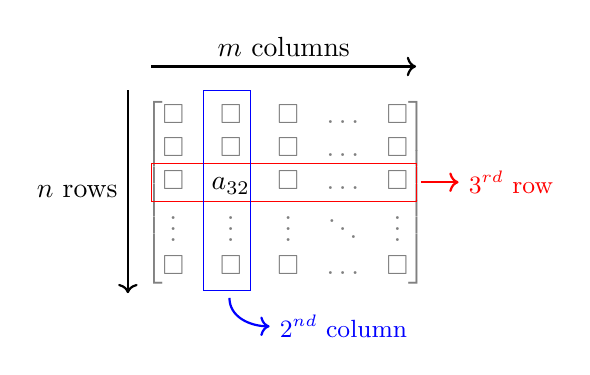
\begin{tikzpicture}[scale=0.6]
\draw[thick, ->] (0,0) -- (0, -4.3) node[midway,left] {$n$ rows};
\draw[thick, ->] (0.5,0.5) -- (6.1, 0.5) node[midway,above]{$m$ columns};
%\node[xshift=-0.6cm,yshift=-1.3cm] {Rows};
\node[gray,xshift=2.0cm,yshift=-1.3cm] {$\begin{bmatrix}
\Box & \Box & \Box & \ldots & \Box \\
\Box & \Box & \Box & \ldots & \Box \\
\Box & \textcolor{black}{a_{32}} & \Box & \ldots & \Box \\
\vdots & \vdots & \vdots & \ddots & \vdots \\
\Box & \Box & \Box & \ldots & \Box \\
\end{bmatrix}$};
\draw[draw=red] (0.5,-2.35) rectangle ++(5.6,0.8);
\draw[draw=blue] (1.6,-4.25) rectangle ++(1.0,4.25);
\draw [thick, blue, ->] (2.15,-4.4) to [out=-90,in=180] (3.0, -5.0) node[right] {\small{$2^{nd}$ column}};
\draw [thick, red, ->] (6.2,-1.95) to (7.,-1.95) node[right] {\small{$3^{rd}$ row}};
\end{tikzpicture}\hspace{0.5cm}
\end{center}
\item Consider a matrix $A$ with $n$ rows and $m$ columns.$ \begin{cases} \text{\textbf{Tall/Skinny}} & n > m\\
\text{\textbf{Square}} & n = m\\
\text{\textbf{Wide/Fat}} & n < m\\
\end{cases}$
\end{itemize}
\end{frame}

\begin{frame}[t]{Matrices}
\begin{itemize}
    \item $n$-vectors can be interpreted as $n \times 1$ matrices. These are called \textit{column vectors}.
    \item A matrix with only one row is called a \textit{row vector}, which can be referred to as $n$-row-vector.  $\mf{x} = \begin{bmatrix}1.45 & -3.1 & 12.4\end{bmatrix}$
    \item\textbf{Block matrices} \& \textbf{Submatrices}: $\mf{A} = \begin{bmatrix}
    \mf{B} & \mf{C} \\
    \mf{D} & \mf{E}
    \end{bmatrix}$.  What are the dimensions of the different matrices?
    \item Matrices are also compact way to give a set of indexed column $n$-vectors, 
    $\mf{x}_1, \mf{x}_2, \mf{x}_3 \ldots \mf{x}_m$. 
    $$\mf{X} = \begin{bmatrix}
    \mf{x}_1 & \mf{x}_2 & \mf{x}_3 & \ldots & \mf{x}_m
    \end{bmatrix}$$
    \item \textbf{Zero matrix}$ = \mf{0}_{n\times m} = \begin{bmatrix}
    0 & 0 & \ldots & 0\\
    0 & 0 & \ldots & 0\\
    \vdots & \vdots & \ddots & \vdots\\
    0 & 0 & \ldots & 0
    \end{bmatrix}$
\end{itemize}
\end{frame}

\begin{frame}[t]{Matrices}
\begin{itemize}
\item \textbf{Identity matrix} is a square $n \times n$ matrix with all zero elements, except the diagonals where all elements are 1.
$$\mf{I}_{ij} = \begin{cases}
1 & i = j\\
0 & i \neq j
\end{cases} \,\,\,\,\,\,\,\, \mf{I}_3=\begin{bmatrix}
1 & 0 & 0\\
0 & 1 & 0\\
0 & 0 & 1\\
\end{bmatrix} = \begin{bmatrix}
\mf{e}_1 & \mf{e}_2 & \mf{e}_3
\end{bmatrix}$$
\item \textbf{Diagonal matrices} is a square matrix with non-zero elements on its diagonal.
$$\begin{bmatrix}
0.4 & 0 & 0 & 0\\
0 & -11 & 0 & 0\\
0 & 0 & 21 & 0\\
0 & 0 & 0 & 9.3\\
\end{bmatrix} = \text{\textbf{diag}}\left(0.4, -11, 21, 9.3\right)$$
\item \textbf{Triangular matrices}: Are square matrices. \textit{Upper triangular} $a_{ij} = 0, \forall i > j$; \textit{Lower triangular} $a_{ij} = 0, \forall i < j$.
\end{itemize}
\end{frame}

\begin{frame}[t]{Matrix operations}
\begin{itemize}
\item \textbf{Transpose} switches the rows and columns of a matrix. $\mf{A}$ is a $n\times m$ matrix, then its transpose is represented by $\mf{A}^T$, which is a $m \times n$ matrix.
\[ \mf{A} = \begin{bmatrix}
a_{11} & a_{12} & a_{13}\\
a_{21} & a_{22} & a_{23}\\
\end{bmatrix} \implies \mf{A}^T = \begin{bmatrix}
a_{11} & a_{21}\\
a_{12} & a_{22}\\
a_{13} & a_{23}\\
\end{bmatrix} \]
Transpose converts between column and row vectors.\\
What is the transpose of a block matrix? $\mf{A} = \begin{bmatrix}
\mf{B} & \mf{C}\\\mf{D} & \mf{E}
\end{bmatrix}$
\item \textbf{Matrix addition} can only be carried out with matrices of same size. Like vectors we perform element wise addition.
\[ \begin{bmatrix}
a_{11} & a_{12}\\
a_{21} & a_{22}\\
\end{bmatrix} + \begin{bmatrix}
b_{11} & b_{12}\\
b_{21} & b_{22}\\
\end{bmatrix} = \begin{bmatrix}
a_{11} + b_{11} & a_{12} + b_{12}\\
a_{21} + b_{21} & a_{22} + b_{22}\\
\end{bmatrix}\]
\end{itemize}
\end{frame}

\begin{frame}[t]{Matrix operations}
\begin{itemize}
\item \textbf{Properties of matrix addition}:
\begin{itemize}
\item \textit{Commutative}: $\mf{A} + \mf{B} = \mf{B} + \mf{A}$
\item \textit{Associative}: $\left(\mf{A} + \mf{B}\right) + \mf{C} = \mf{A} + \left(\mf{B} + \mf{C}\right)$
\item \textit{Addition with zero matrix}: $\mf{A} + \mf{0} = \mf{0} + \mf{A} = \mf{A}$
\item \textit{Transpose of sum}: $\left(\mf{A} + \mf{B}\right)^T = \mf{A}^T + \mf{B}^T$
\end{itemize}
\item \textbf{Scalar multiplication} Each element of the matrix gets multiplied by the scalar.
\[ \alpha \begin{bmatrix}
a_{11} & a_{12}\\
a_{21} & a_{22}\\
\end{bmatrix} = \begin{bmatrix}
\alpha a_{11} & \alpha a_{12} \\
\alpha a_{21} & \alpha a_{22} \\
\end{bmatrix}\]
\item We will mostly only deal with matrices with real entries. Such matrices are elements of the set $\mathbb{R}^{n\times m}$.
\item Given the aforementioned matrix operations and their properties, is $\mathbb{R}^{n\times m}$ a vector space?
\end{itemize}
\end{frame}

\begin{frame}[t]{Matrix multiplication}
\begin{itemize}
\item It is possible to \textit{multiply} two matrices $\mf{A} \in \mathbb{R}^{n\times p}$ and $\mf{B} \in \mathbb{R}^{p\times m}$ through \textit{matrix multiplication} procedure.
\item There is a product matrix $\mf{C} \coloneqq \mf{A}\mf{B} \in \mathbb{R}^{n \times m}$, if the number of columns of $\mf{A}$ is equal to the number of rows of $\mf{B}$.
\[ c_{ij} \coloneqq \sum_{k=1}^{p} a_{ik}b_{kj} \,\,\,\,\, \forall i \in \left\{1, \ldots n\right\} \,\,\, \& \,\,\, j \in \left\{1 \ldots m\right\} \]
\item \textit{Inner product} is a special case of matrix multiplication between a \textit{row vector} and a \textit{column vector}.
\[ \mf{x}^T\mf{y} = \begin{bmatrix}
x_1 \\ x_2 \\ \vdots \\x_n
\end{bmatrix}^T\begin{bmatrix}
y_1 \\ y_2 \\ \vdots \\y_n
\end{bmatrix} = \begin{bmatrix}
x_1 & x_2 & \ldots &x_n
\end{bmatrix}\begin{bmatrix}
y_1 \\ y_2 \\ \vdots \\y_n
\end{bmatrix} = \sum_{i=1}^nx_iy_i\]
\end{itemize}
\end{frame}

\begin{frame}[t]{Matrix multiplication}
\begin{itemize}
\item Consider a matrix $\mf{A} \in \mathbb{R}^{n \times m}$ and a $m$-vector $\mf{x} \in \mathbb{R}^m$. We can multiply $\mf{A}$ and $\mf{x}$ to obtain $\mf{y} = \mf{A}\mf{x} \in \mathbb{R}^n$.
\[ \mf{y} = \begin{bmatrix}
a_{11} & a_{12} & \ldots & a_{1m} \\
a_{21} & a_{22} & \ldots & a_{2m} \\
\vdots & \vdots & \ddots & \vdots \\
a_{n1} & a_{n2} & \ldots & a_{nm} \\
\end{bmatrix}\begin{bmatrix}
x_1\\ x_2 \\ \vdots \\ x_{m}
\end{bmatrix} = \begin{bmatrix}
\tilde{\mf{a}}_1^T\\ \tilde{\mf{a}}_2^T \\ \vdots \\ \tilde{\mf{a}}_n^T
\end{bmatrix}x = \begin{bmatrix}
\tilde{\mf{a}}_{1}^Tx\\ \tilde{\mf{a}}_2^Tx \\ \vdots \\ \tilde{\mf{a}}_n^Tx
\end{bmatrix} = \begin{bmatrix}
\sum_{i=1}^ma_{1i}x_i\\ \sum_{i=1}^ma_{2i}x_i \\ \vdots \\ \sum_{i=1}^ma_{ni}x_i
\end{bmatrix} \]
\[ \mf{y} = \sum_{i=1}^mx_i\begin{bmatrix}
a_{1i} \\ a_{2i} \\ \vdots \\ a_{ni}
\end{bmatrix} = x_1\begin{bmatrix}
a_{11} \\ a_{21} \\ \vdots \\ a_{n1}
\end{bmatrix} + x_2 \begin{bmatrix}
a_{12} \\ a_{22} \\ \vdots \\ a_{n2}
\end{bmatrix} + \ldots + x_m \begin{bmatrix}
a_{1m} \\ a_{2m} \\ \vdots \\ a_{nm}
\end{bmatrix} \]
\item Multiplying a matrix $\mf{A}$ by a column vector $\mf{x}$ produces a linear combination of the columns of matrix $\mf{A}$. The column mixture is provided by $\mf{x}$.
\end{itemize}
\end{frame}

\begin{frame}[t]{Matrix multiplication}
\begin{itemize}
\item We see a similar process in play when we multiply a row vector $\mf{x}^T \in \mathbb{R}^{n}$ by a matrix $\mf{A} \in \mathbb{R}^{n \times m}$.
\[ \mf{y} = \mf{x}^T\mf{A} = \begin{bmatrix}
x_1\\ x_2 \\ \vdots \\ x_n
\end{bmatrix}^T\begin{bmatrix}
a_{11} & a_{12} & \ldots & a_{1m} \\
a_{21} & a_{22} & \ldots & a_{2m} \\
\vdots & \vdots & \ddots & \vdots \\
a_{n1} & a_{n2} & \ldots & a_{nm} \\
\end{bmatrix} = \mf{x}^T\begin{bmatrix}
\mf{a}_1 & \mf{a}_2 & \ldots & \mf{a}_m
\end{bmatrix} \]
\[ \mf{y} = \begin{bmatrix}
\mf{x}^T\mf{a}_1 & \mf{x}^T\mf{a}_2 & \ldots & \mf{x}^T\mf{a}_m\end{bmatrix} = \sum_{i=1}^{n}x_i\begin{bmatrix}
a_{i1} & a_{i2} & \ldots & a_{im}\end{bmatrix} \]
\item Multiplying a row vector $\mf{x}$ by a matrix $\mf{A}$ produces a linear combination of the row of matrix $\mf{A}$. The row mixture is provided by $\mf{x}$.
\end{itemize}
\end{frame}

\begin{frame}[t]{Matrix multiplication}
\begin{itemize}
\item Multiplying two matrices $\mf{A} \in \mathbb{R}^{n \times p}$ and $\mf{B} \in \mathbb{R}^{p \times m}$, we have $\mf{C} \in \mathbb{R}^{n \times m}$,
\[ \mf{C} = \mf{A}\mf{B} = \begin{bmatrix}
a_{11} & a_{12} & \ldots & a_{1p} \\
a_{21} & a_{22} & \ldots & a_{2p} \\
\vdots & \vdots & \ddots & \vdots \\
a_{n1} & a_{n2} & \ldots & a_{np} \\
\end{bmatrix} \begin{bmatrix}
b_{11} & b_{12} & \ldots & b_{1m} \\
b_{21} & b_{22} & \ldots & b_{2m} \\
\vdots & \vdots & \ddots & \vdots \\
b_{p1} & b_{p2} & \ldots & b_{pm} \\
\end{bmatrix} = \begin{bmatrix}
c_{11} & c_{12} & \ldots & c_{1m} \\
c_{21} & c_{22} & \ldots & c_{2m} \\
\vdots & \vdots & \ddots & \vdots \\
c_{p1} & c_{n2} & \ldots & c_{nm} \\
\end{bmatrix}\]
\item \textbf{Inner product interpretation}: $c_{ij} = \tilde{\mf{a}}_i^T\mf{b}_j, \, i \in \left\{1 \ldots n\right\}, j \in \left\{1 \ldots m\right\}$
\item \textbf{Column interpretation}: $\mf{C} = \mf{A} \begin{bmatrix}
\mf{b}_{1} & \mf{b}_{2} & \ldots & \mf{b}_{m}
\end{bmatrix} = \begin{bmatrix}
\mf{A}\mf{b}_{1} & \mf{A}\mf{b}_{2} & \ldots & \mf{A}\mf{b}_{m}
\end{bmatrix}$
\item \textbf{Row interpretation} : $\mf{C} = \begin{bmatrix}
\tilde{\mf{a}}_{1}^T\\
\tilde{\mf{a}}_{2}^T\\
\vdots\\
\tilde{\mf{a}}_{n}^T\\
\end{bmatrix} \mf{B} = \begin{bmatrix}
\tilde{\mf{a}}_{1}^T\mf{B}\\
\tilde{\mf{a}}_{2}^T\mf{B}\\
\vdots\\
\tilde{\mf{a}}_{n}^T\mf{B}\\
\end{bmatrix}$
\end{itemize}
\end{frame}

\begin{frame}[t]{Matrix multiplication}
\begin{small}
\begin{itemize}
    \item \textbf{Outer product interpretation} Consider two $n$-vectors $\mf{x}, \mf{y} \in \mathbb{R}^n$. The \textit{outer product} is defined as,
    \[ \mf{x}\mf{y}^T = \begin{bmatrix}
    x_1\\ x_2\\ x_3\\ \vdots \\x_n
    \end{bmatrix} \begin{bmatrix}
    y_1 &  y_2 & y_3 & \ldots & y_n
    \end{bmatrix} = \begin{bmatrix}
    x_1y_1 &  x_1y_2 & x_1y_3 & \ldots & x_1y_n \\
    x_2y_1 &  x_2y_2 & x_2y_3 & \ldots & x_2y_n \\
    x_3y_1 &  x_3y_2 & x_3y_3 & \ldots & x_3y_n \\
    \vdots &  \vdots & \vdots & \ddots & \vdots \\
    x_ny_1 &  x_ny_2 & x_ny_3 & \ldots & x_ny_n \\
    \end{bmatrix} \]
    \item We can represent the product between two matrices as the sum of outer products between the columns and $\mf{A}$ and rows of $\mf{B}$. 
    \[ \mf{A}\mf{B} = \begin{bmatrix}
    \mf{a}_1 & \mf{a}_2 & \mf{a}_3 & \ldots & \mf{a}_p
    \end{bmatrix} \begin{bmatrix}
    \tilde{\mf{b}}_1^T \\
    \tilde{\mf{b}}_2^T \\
    \tilde{\mf{b}}_3^T \\
    \vdots \\
    \tilde{\mf{b}}_p^T
    \end{bmatrix} = \sum_{i=1}^{p}a_i\tilde{b}_i^T \]
\end{itemize}
\end{small}
\end{frame}

\begin{frame}[t]{Properties of matrix multiplication}
\begin{itemize}
\item \textbf{Not commutative}: $\mf{A}\mf{B} \neq \mf{B}\mf{A}$\\
The product of two matrices might not alwasys be defined. When it is defined, $\mf{A}\mf{B}$ and $\mf{B}\mf{A}$ need not match.
\item \textbf{Distributive}:  $\mf{A}\left(\mf{B} + \mf{C}\right) = \mf{A}\mf{B} + \mf{B}\mf{C}$ and $\left(\mf{A} + \mf{B}\right)\mf{C} = \mf{A}\mf{C} + \mf{B}\mf{C}$ 
\item \textbf{Associative}: $\mf{A}\left(\mf{B}\mf{C}\right) = \left(\mf{A}\mf{B}\right)\mf{C} $
\item \textbf{Transpose}: $\left(\mf{A}\mf{B}\right)^T = \mf{B}^T\mf{A}^T$
\item \textbf{Scalar product}: $\alpha\left(\mf{A}\mf{B}\right) = \left(\alpha \mf{A}\right)\mf{B} = \mf{A}\left(\alpha \mf{B}\right)$
\end{itemize}
\end{frame}

\begin{frame}[t]{Linear equations}
\begin{itemize}
\item Matrices present a compact way to represent a set of linear equations. Consider the following,
\[
\begin{rcases*}
\begin{split}
a_{11}x_1 + a_{12}x_2 \ldots + a_{1n}x_n & = b_1 \\
a_{21}x_1 + a_{22}x_2 \ldots + a_{2n}x_n & = b_2 \\
a_{31}x_1 + a_{32}x_2 \ldots + a_{3n}x_n & = b_3 \\
\vdots \\
a_{m1}x_1 + a_{m2}x_2 \ldots + a_{mn}x_n & = b_m \\
\end{split}
\end{rcases*} \, \longrightarrow \mf{Ax} = \mf{b}, \,\,\, \mf{A} \in \mathbb{R}^{m \times n}, \,\, \mf{x} \in \mathbb{R}^n, \,\, \mf{b} \in \mathbb{R}^m
\]

\[
\mf{A} = \begin{bmatrix}
a_{11} & a_{12} & a_{13} & \ldots & a_{1n}\\
a_{21} & a_{22} & a_{23} & \ldots & a_{2n}\\
\vdots & \vdots & \vdots & \ddots & \vdots\\
a_{m1} & a_{m2} & a_{m3} & \ldots & a_{mn}\\
\end{bmatrix} \,\,\,\,\, 
\mf{x} = \begin{bmatrix}
x_1\\ x_2\\ \vdots \\ x_n
\end{bmatrix} \,\,\,\,\,
\mf{b} = \begin{bmatrix}
b_1\\ b_2\\ \vdots \\ b_m
\end{bmatrix}
\]
\end{itemize}
\end{frame}

\begin{frame}[t]{Geometry of linear equations}
\vspace{-0.5cm}
\[\begin{rcases*}
\begin{split} x_1 + 2x_2 &= -1 \\ x_1 + x_2 &= 1 \end{split}
\end{rcases*} \longrightarrow \begin{bmatrix}
1 & 2\\
1 & 1
\end{bmatrix}\begin{bmatrix}
x_1\\
x_2
\end{bmatrix} = \begin{bmatrix}
-1\\
1
\end{bmatrix}\]
Two ways to view this: \textbf{row view} and the \textbf{column view}.
\begin{center}
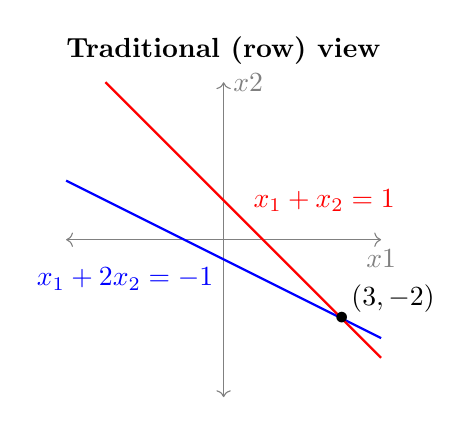
\begin{tikzpicture}[scale=0.5]
\node[yshift=2.4cm] {\textbf{Traditional (row) view}};
\draw[gray,<->] (-4, 0) -- (4, 0) node[right,below] {$x1$};
\draw[gray,<->] (0, -4) -- (0, 4) node[right] {$x2$};
\draw[blue,thick] (-4,3/2) -- (4, -5/2) node[midway,left,yshift=-0.25cm] {$x_1 + 2x_2 = -1$};
\draw[red,thick] (-3,4) -- (4, -3) node[midway,right,yshift=0.25cm] {$x_1 + x_2 = 1$};
\draw (3,-2) node[] {$\bullet$};
\draw (3,-2) node[right,yshift=0.25cm] {$\left(3,-2\right)$};
\end{tikzpicture}\hspace{1cm}
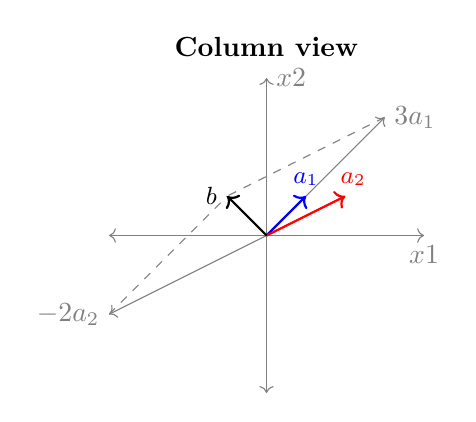
\begin{tikzpicture}[scale=0.5]
\node[yshift=2.4cm] {\textbf{Column view}};
\draw[gray,<->] (-4, 0) -- (4, 0) node[right,below] {$x1$};
\draw[gray,<->] (0, -4) -- (0, 4) node[right] {$x2$};
\draw[gray,thin,->] (0,0) -- (3,3) node[above,right] {$3a_1$};
\draw[blue,thick,->] (0,0) -- (1,1) node[above,yshift=0.cm] {\small{$a_1$}};
\draw[red,thick,->] (0,0) -- (2,1) node[above,xshift=0.1cm,yshift=0.cm] {\small{$a_2$}};
\draw[gray,thin,->] (0,0) -- (-4,-2) node[below,left] {$-2a_2$};
\draw[gray,thin,dashed] (3,3) -- (-1,1);
\draw[gray,thin,dashed] (-4,-2) -- (-1,1);
\draw[black,thick,->] (0,0) -- (-1,1) node[above,left] {\small{$b$}};

\end{tikzpicture}
\end{center}
\end{frame}

\begin{frame}[t]{Solving linear equations}
\vspace{-0.5cm}
$$ \mf{Ax = b}, \,\,\, \mf{A} \in \mathbb{R}^{m \times n}, \,\, \mf{x} \in \mathbb{R}^n, \,\, \mf{b} \in \mathbb{R}^m$$
\vspace{-0.5cm}
\begin{itemize}
\item \textbf{Three possible situations:} \textsc{No solution}, \textsc{Infinitely many solutions}, or \textsc{Unique Solution}.
\item When do have infinitely many or no solutions? In $\mathbb{R}^3$, we can visualize the different situations.
\end{itemize}
\begin{center}
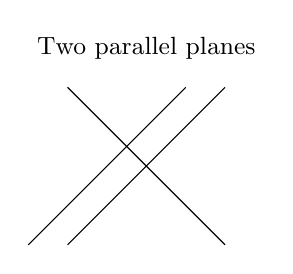
\begin{tikzpicture}[scale=0.5]
\node[yshift=1.5cm] {\small{Two parallel planes}};
\draw[black,-] (-2, -2) -- (2, 2);
\draw[black,-] (-3, -2) -- (1, 2);
\draw[black,-] (2, -2) -- (-2, 2);
\end{tikzpicture}\hspace{0.25cm}
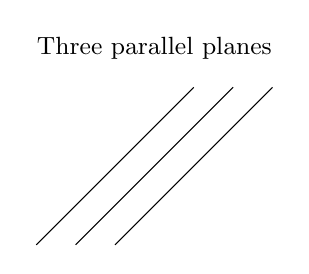
\begin{tikzpicture}[scale=0.5]
\node[yshift=1.5cm] {\small{Three parallel planes}};
\draw[black,-] (-2, -2) -- (2, 2);
\draw[black,-] (-3, -2) -- (1, 2);
\draw[black,-] (-1, -2) -- (3, 2);
\end{tikzpicture}\hspace{0.25cm}
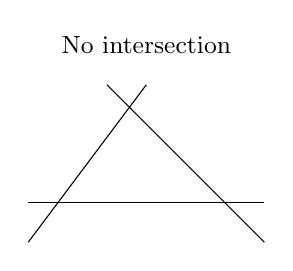
\begin{tikzpicture}[scale=0.5]
\node[yshift=1.0cm] {\small{No intersection}};
\draw[black,-] (-3, -2) -- (3, -2);
\draw[black,-] (-3, -3) -- (0, 1);
\draw[black,-] (3, -3) -- (-1, 1);
\end{tikzpicture}\hspace{0.25cm}
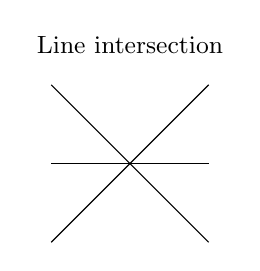
\begin{tikzpicture}[scale=0.5]
\node[yshift=1.5cm] {\small{Line intersection}};
\draw[black,-] (-2, 0) -- (2, 0);
\draw[black,-] (-2, -2) -- (2, 2);
\draw[black,-] (2, -2) -- (-2, 2);
\end{tikzpicture}
\end{center} 
\end{frame}

\begin{frame}[t]{Solving linear equations: Gaussian Elimination}
\vspace{-0.5cm}
\begin{small}
\[
\begin{split}
a_{11}x_1 + a_{12}x_2 \ldots + a_{1n}x_n & = b_1: E_1 \\
a_{21}x_1 + a_{22}x_2 \ldots + a_{2n}x_n & = b_2: E_2 \\
a_{31}x_1 + a_{32}x_2 \ldots + a_{3n}x_n & = b_3: E_3 \\
\vdots \\
a_{m1}x_1 + a_{m2}x_2 \ldots + a_{mn}x_n & = b_m: E_m \\
\end{split}
\]
\end{small}
\vspace{-0.5cm}

\begin{itemize}
\item Gaussian elimination is a systematic way of simplifying the above equations to an equivalent system that can be easily solved.  
\item Three simple operations are repeatedly performed:
\begin{itemize}
\item Interchanging of equations $E_i$ and $E_j$.
\item Replacing equation $E_i$ by $\alpha E_i$, $\alpha \neq 0$.
\item Replacing equation $E_j$ by $E_j + \alpha E_i$, $\alpha \neq 0$.
\end{itemize}
\item These three operations do not change the solution of the given linear system.
\end{itemize}
\end{frame}

\begin{frame}[t]{Solving linear equations: Gaussian Elimination}
\begin{center}
\textbf{Augmented matrix}: $\left[
\begin{array}{cccc|c}
a_{11} & a_{12} & \cdots & a_{1n} & b_1 \\
a_{21} & a_{22} & \cdots & a_{2n} & b_2 \\
a_{31} & a_{32} & \cdots & a_{3n} & b_3 \\
\vdots & \vdots & \ddots & \vdots & \vdots \\
a_{m1} & a_{m2} & \cdots & a_{mn} & b_m \\
\end{array}
\right]$
\vspace{0.5cm}
\begin{itemize}
\item We can work with the augmented matrix instead of the equations.
\item Gaussian elimination is carried out on the entire matrix.
\item The matrix is simplified to a point, from where one can easily:
\begin{itemize}
\item find out the nature of the solutions for the system of equations; and
\item find the solution (with a bit of extra work), if they exist.
\end{itemize}
\end{itemize}
\end{center}
\end{frame}

\begin{frame}[t]{Solving linear equations: Gaussian Elimination}
\begin{small}
\[
\begin{rcases*}
\begin{array}{rrrrrrr}
x_1 &+& 2x_2 &-& x_3 & =& 1 \\
2x_1 &+& 3x_2 &+& 4x_3  & =& 4 \\
-2x_1 &-& 4x_2 &+& x_3  & =& -3 \\
\end{array}
\end{rcases*} \, \longrightarrow \left[
\begin{array}{rrr|r}
1& 2 & -1 & 1 \\
2 & 3 & 4 & 4 \\
-2 & -4 & 1 & -3 \\
\end{array}
\right]
\]
\end{small}

\noindent \textbf{Gaussian Elimination}
\begin{small}
\[
\left[
\begin{array}{rrr|r}
\color{red}{\underline{1}} & 2 & -1 & 1 \\
2 & 3 & 4 & 4 \\
-2 & -4 & 1 & -3 \\
\end{array}
\right] \longrightarrow
\left[
\begin{array}{rrr|r}
\color{red}{\underline{1}} & 2 & -1 & 1 \\
0 & -1 & 6 & 2 \\
-2 & -4 & 1 & -3 \\
\end{array}
\right] \longrightarrow
\left[
\begin{array}{rrr|r}
\color{red}{\underline{1}} & 2 & -1 & 1 \\
0 & \color{red}{\underline{-1}} & 6 & 2 \\
0 & 0 & \color{red}{\underline{-1}} & -1 \\
\end{array}
\right]
\]
\end{small}

\noindent Now, we can perform \textbf{back substitution} on this triangularized system of linear equations,
\[ x_3 = 1; \,\,\, x_2 = 4; \,\,\, x_1 = -6 \]

We can continue the simplification process through the \textbf{Gauss-Jordan} method.
\end{frame}

\begin{frame}[t]{Solving linear equations: Gauss-Jordan Method}
\noindent Continue the elimination upwards until all elements, except the ones in the main diagonal, are zero.
\begin{small}
\[
\left[
\begin{array}{rrr|r}
1 & 2 & -1 & 1 \\
0 & -1 & 6 & 2 \\
0 & 0 & -1 & -1 \\
\end{array}
\right] \longrightarrow
\left[
\begin{array}{rrr|r}
1 & 2 & -1 & 1 \\
0 & -1 & 0 & -4 \\
0 & 0 & 1 & 1 \\
\end{array}
\right] \longrightarrow
\left[
\begin{array}{rrr|r}
1 & 2 & -1 & 1 \\
0 & 1 & 0 & 4 \\
0 & 0 & 1 & 1 \\
\end{array}
\right] \longrightarrow
\left[
\begin{array}{rrr|r}
1 & 2 & 0 & 2 \\
0 & 1 & 0 & 4 \\
0 & 0 & 1 & 1 \\
\end{array}
\right]
\]
\[
\left[
\begin{array}{rrr|r}
1 & 2 & 0 & 2 \\
0 & 1 & 0 & 4 \\
0 & 0 & 1 & 1 \\
\end{array}
\right] \longrightarrow
\left[
\begin{array}{rrr|r}
1 & 0 & 0 & -6 \\
0 & 1 & 0 & 4 \\
0 & 0 & 1 & 1 \\
\end{array}
\right] \implies x_1 = -6; \,\,\, x_2 = 4; \,\,\, x_3 = 1; 
\]
\end{small}

\noindent Everything worked out well without any problems. What can go wrong here?
\vspace{0.25cm}

Try solving the these systems, $\left[\begin{array}{rrr|r}
1 & 2 & -1 & 1 \\
2 & 3 & 4 & 4 \\
-2 & -4 & 2 & -3 \\
\end{array}\right]
$, $\left[\begin{array}{rrr|r}
1 & 2 & -1 & 1 \\
2 & 3 & 4 & 4 \\
-2 & -4 & 2 & -2 \\
\end{array}\right]
$
\vspace{0.25cm}

What is the difference between these two systems?
\end{frame}

\begin{frame}[t]{Solving linear equations: Rectangular systems and Row Echelon Form}
\vspace{-0.5cm}
\begin{small}
\[
\begin{split}
a_{11}x_1 + a_{12}x_2 \ldots + a_{1n}x_n & = b_1 : E_1\\
a_{21}x_1 + a_{22}x_2 \ldots + a_{2n}x_n & = b_2 : E_2\\
a_{31}x_1 + a_{32}x_2 \ldots + a_{3n}x_n & = b_3 : E_3\\
\vdots &  \\
a_{m1}x_1 + a_{m2}x_2 \ldots + a_{mn}x_n & = b_m : E_m\\
\end{split} \longrightarrow
\left[
\begin{array}{cccc|c}
a_{11} & a_{12} & \cdots & a_{1n} & b_1 \\
a_{21} & a_{22} & \cdots & a_{2n} & b_2 \\
a_{31} & a_{32} & \cdots & a_{3n} & b_3 \\
\vdots & \vdots & \ddots & \vdots & \vdots \\
a_{m1} & a_{m2} & \cdots & a_{mn} & b_m \\
\end{array}
\right]
\]
\end{small}

Consider the following example,
\begin{footnotesize}
\[
\left[
\begin{array}{rrrrr|r}
\color{red}{\underline{1}} & -2 & 1 & 0 & 1 & 1 \\
2 & -4 & 1 & -1 & -2 & 2 \\
-1 & 2 & 1 & 1 & 2 & -1 \\
\end{array}
\right] \longrightarrow 
\left[
\begin{array}{rrrrr|r}
\color{red}{\underline{1}} & -2 & 1 & 0 & 1 & 1 \\
0 & 0 & \color{red}{\underline{-1}} & -1 & -4 & 0 \\
0 & 0 & 2 & 1 & 3 & 0 \\
\end{array}
\right] \longrightarrow 
\left[
\begin{array}{rrrrr|r}
\color{red}{\underline{1}} & -2 & 1 & 0 & 1 & 1 \\
0 & 0 & \color{red}{\underline{-1}} & -1 & -4 & 0 \\
0 & 0 & 0 & \color{red}{\underline{-1}} & -5 & 0 \\
\end{array}
\right]
\]
\end{footnotesize}
\end{frame}

\begin{frame}[t]{Solving linear equations: Rectangular systems and Row Echelon Form}
\vspace{-0.5cm}
\begin{small}
\[
\left[
\begin{array}{cccc|c}
a_{11} & a_{12} & \cdots & a_{1n} & b_1 \\
a_{21} & a_{22} & \cdots & a_{2n} & b_2 \\
a_{31} & a_{32} & \cdots & a_{3n} & b_3 \\
\vdots & \vdots & \ddots & \vdots & \vdots \\
a_{m1} & a_{m2} & \cdots & a_{mn} & b_m \\
\end{array}
\right] \longrightarrow
\left[
\begin{array}{cccccccc}
\color{red}{\underline{\ast}} & \ast & \ast & \ast & \ast & \ast & \ast \\
0 & 0 & \color{red}{\underline{\ast}}  & \ast  & \ast  & \ast  & \ast \\
0 & 0 & 0 & \color{red}{\underline{\ast}}  & \ast  & \ast  & \ast \\
0 & 0 & 0 & 0 & \color{red}{\underline{\ast}}  & \ast  & \ast \\
0 & 0 & 0 & 0 & 0 & 0 & \color{red}{\underline{\ast}} \\
0 & 0 & 0 & 0 & 0 & 0 & 0 \\
\end{array}
\right]
\]
\textbf{Things to notice about the echelon form:}
\begin{itemize}
\item If a particualr row consists entirely of zeros, then all rows below that row also contain entirely of zeros.
\item If the first non-zero entry in the $i^{th}$ row occurs in the $j^{th}$ position, then all elements below the $i^{th}$ row are zero from columns $1$ to $j$.
\end{itemize}

Columns containing pivot are called the \textbf{\textit{basic columns}}.
\end{small}

\begin{tcolorbox}[colback=gray!20,colframe=black]
\textbf{Rank of a matrix $\mf{A}$} is defined at the number of basic columns in the row echelon form of the matrix $\mf{A}$.
\end{tcolorbox}
\end{frame}

\begin{frame}[t]{Solving linear equations: Reduced Row Echelon Form}
\vspace{-0.5cm}
\begin{footnotesize}
\[
\left[
\begin{array}{cccccccc}
\color{red}{\underline{\ast}} & \ast & \ast & \ast & \ast & \ast & \ast \\
0 & 0 & \color{red}{\underline{\ast}}  & \ast  & \ast  & \ast  & \ast \\
0 & 0 & 0 & \color{red}{\underline{\ast}}  & \ast  & \ast  & \ast \\
0 & 0 & 0 & 0 & \color{red}{\underline{\ast}}  & \ast  & \ast \\
0 & 0 & 0 & 0 & 0 & 0 & \color{red}{\underline{\ast}} \\
0 & 0 & 0 & 0 & 0 & 0 & 0 \\
\end{array}
\right] \xrightarrow[\text{}]{\text{Gauss-Jordan}}
\left[
\begin{array}{cccccccc}
\color{red}{\underline{1}} & \ast & 0 & 0  & 0 & \ast & 0 \\
0 & 0 & \color{red}{\underline{1}}  & 0 & 0 & \ast & 0 \\
0 & 0 & 0 & \color{red}{\underline{1}}  & 0 & \ast  & 0 \\
0 & 0 & 0 & 0 & \color{red}{\underline{1}}  & \ast  & 0 \\
0 & 0 & 0 & 0 & 0 & 0 & \color{red}{\underline{1}} \\
0 & 0 & 0 & 0 & 0 & 0 & 0 \\
\end{array}
\right]
\]
\end{footnotesize}
\vspace{-0.05cm}
\begin{footnotesize}
\[
\left[
\begin{array}{rrrrr|r}
\color{red}{\underline{1}} & -2 & 1 & 0 & 1 & 1 \\
0 & 0 & \color{red}{\underline{-1}} & -1 & -4 & 0 \\
0 & 0 & 0 & \color{red}{\underline{-1}} & -5 & 0 \\
\end{array}
\right] \longrightarrow
\left[
\begin{array}{rrrrr|r}
\color{red}{\underline{1}} & -2 & 0 & -1 & -3 & 1 \\
0 & 0 & \color{red}{\underline{1}} & 1 & 4 & 0 \\
0 & 0 & 0 & \color{red}{\underline{-1}} & -5 & 0 \\
\end{array}
\right] \longrightarrow 
\left[
\begin{array}{rrrrr|r}
\color{red}{\underline{1}} & -2 & 0 & 0 & 2 & 1 \\
0 & 0 & \color{red}{\underline{1}} & 0 & -1 & 0 \\
0 & 0 & 0 & \color{red}{\underline{1}} & 5 & 0 \\
\end{array}
\right]
\]
\end{footnotesize}
\vspace{-0.1cm}
\begin{small}
\begin{itemize}
\item All non-basic columns can be represented as a linear combination of the basic columns.
\item A non-basic columns is a linear  combination of only the columns before it.
\item Scaling factors for each basic comlumns is determined by the corresponding elements of the non-basic columns.
\end{itemize}
\end{small}

\begin{small}
\begin{tcolorbox}[colback=gray!20,colframe=black]
\begin{center}
\textbf{The reduced row echelon form reveals structure in the original matrix $\mf{A}$.}
\end{center}
\end{tcolorbox}
\end{small}
\end{frame}

\begin{frame}[t]{Solving linear equations: Homogenous Systems}
\vspace{-0.75cm}
\begin{footnotesize}
\[
\begin{split}
a_{11}x_1 + a_{12}x_2 \ldots + a_{1n}x_n & = 0\\
a_{21}x_1 + a_{22}x_2 \ldots + a_{2n}x_n & = 0\\
a_{31}x_1 + a_{32}x_2 \ldots + a_{3n}x_n & = 0\\
\vdots &  \\
a_{m1}x_1 + a_{m2}x_2 \ldots + a_{mn}x_n & = 0\\
\end{split} \longrightarrow
\left[
\begin{array}{cccc|c}
a_{11} & a_{12} & \cdots & a_{1n} & 0 \\
a_{21} & a_{22} & \cdots & a_{2n} & 0 \\
a_{31} & a_{32} & \cdots & a_{3n} & 0 \\
\vdots & \vdots & \ddots & \vdots & \vdots \\
a_{m1} & a_{m2} & \cdots & a_{mn} & 0 \\
\end{array}
\right]
\]
\end{footnotesize}
\vspace{-0.1cm} 

\begin{scriptsize}
Consider the following case,
\vspace{-0.2cm} 

\[
\left[
\begin{array}{rrrrr|r}
1 & -2 & 1 & 0 & 1 & 0 \\
2 & -4 & 1 & -1 & -2 & 0 \\
-1 & 2 & 1 & 1 & 2 & 0 \\
\end{array}
\right] \longrightarrow  
\left[
\begin{array}{rrrrr|r}
1 & -2 &  0 &  0 &  2 &  0 \\
0 &  0 &  1 &  0 & -1 &  0 \\
0 &  0 &  0 &  1 &  5 &  0 \\
\end{array}
\right]
\]
\vspace{-0.75cm}

\[
\begin{split}
x_1 - 2x_2 + 2x_5 & = 0\\
x_3 - x_5 & = 0\\
x_4 + 5x_5 & = 0\\
\end{split} \longrightarrow
\begin{split}
x_1 &=  2x_2 - 2x_5\\
x_3 &=  x_5\\
x_4 &= -5x_5\\
\end{split} \longrightarrow
\begin{bmatrix}
x_1\\ x_2\\ x_3\\ x_4\\ x_5
\end{bmatrix} = \begin{bmatrix}
2x_2 - 2x_5\\ x_2\\ x_5\\ 5x_5\\ x_5
\end{bmatrix} = x_2\begin{bmatrix}
2\\ 1\\ 0\\ 0\\ 0
\end{bmatrix} + x_5\begin{bmatrix}
-2\\ 0\\ 1\\ -5\\ 1
\end{bmatrix}
\]
\end{scriptsize}
\end{frame}


\begin{frame}[t]{Solving linear equations: Homogenous Systems}
\begin{small}
\begin{itemize}
    \item $\begin{bmatrix}x_1\\ x_2\\ x_3\\ x_4\\ x_5\end{bmatrix} = x_2\begin{bmatrix}2\\ 1\\ 0\\ 0\\ 0\end{bmatrix} + x_5\begin{bmatrix}-2\\ 0\\ 1\\ -5\\ 1\end{bmatrix}$ represents the general solution of the system of equations.

    \item In general, any system $\left[ \mf{A} \left|\right.\mf{0}\right]$ with $rank\left(\mf{A}\right) = r$ and $r < n$ has the general solution of the form,
    \[ \mf{x} = x_{f_1} \mf{h}_1 + x_{f_2} \mf{h}_2 + \ldots + x_{f_{n-r}} \mf{h}_{n-r} \]
    where,  the variables $x_{f_1}, x_{f_2}, \ldots , x_{f_{n-r}}$ are called the \textbf{free variables}.
    \item Free variables are the one corresponding to the non-basic columns; the variable variables corresponding to the basic columns are the \textbf{basic variables}.
    \item When does a homogenous system have a unique solution solution? $\longrightarrow rank\left(\mf{A}\right) = n$.
\end{itemize}
\end{small}
\end{frame}

\begin{frame}[t]{Solving linear equations: Non-homogenous Systems}
\vspace{-0.75cm}
\begin{footnotesize}
\[
\begin{split}
a_{11}x_1 + a_{12}x_2 \ldots + a_{1n}x_n & = b_1\\
a_{21}x_1 + a_{22}x_2 \ldots + a_{2n}x_n & = b_2\\
a_{31}x_1 + a_{32}x_2 \ldots + a_{3n}x_n & = b_3\\
\vdots & \\
a_{m1}x_1 + a_{m2}x_2 \ldots + a_{mn}x_n & = b_m\\
\end{split}\longrightarrow \left[ \mf{A} \left|\right.\mf{b}\right]
\]
\end{footnotesize}
\vspace{-0.3cm} 

\begin{scriptsize}
Consider the following case,
\vspace{-0.2cm} 
\[
\left[
\begin{array}{rrrrr|r}
1 & -2 & 1 & 0 & 1 & 1 \\
2 & -4 & 1 & -1 & -2 & 2 \\
-1 & 2 & 1 & 1 & 2 & -1 \\
\end{array}
\right] \longrightarrow  
\left[
\begin{array}{rrrrr|r}
1 & -2 &  0 &  0 &  2 &  1 \\
0 &  0 &  1 &  0 & -1 &  0 \\
0 &  0 &  0 &  1 &  5 &  0 \\
\end{array}
\right]
\]
\vspace{-1.0cm}

\[
\begin{split}
x_1 - 2x_2 + 2x_5 & = 1\\
x_3 - x_5 & = 0\\
x_4 + 5x_5 & = 0\\
\end{split} \longrightarrow
\begin{split}
x_1 &=  1 + 2x_2 - 2x_5\\
x_3 &=  x_5\\
x_4 &= -5x_5\\
\end{split} \longrightarrow
\begin{bmatrix}
x_1\\ x_2\\ x_3\\ x_4\\ x_5
\end{bmatrix} = \begin{bmatrix}
1 + 2x_2 - 2x_5\\ x_2\\ x_5\\ 5x_5\\ x_5
\end{bmatrix} = \begin{bmatrix}
1\\ 0\\ 0\\ 0\\ 0
\end{bmatrix} + x_2\begin{bmatrix}
2\\ 1\\ 0\\ 0\\ 0
\end{bmatrix} + x_5\begin{bmatrix}
-2\\ 0\\ 1\\ -5\\ 1
\end{bmatrix}
\]
\end{scriptsize}
\vspace{-0.3cm}

The general solution of a non-homogenous system is sum of the particular solution and the general solution of the associated homogenous system.
\end{frame}


\begin{frame}[t]{Solving linear equations: Non-homogenous Systems}
\vspace{-0.2cm} 

\begin{scriptsize}
\begin{itemize}
    \item The general solution for $\left[ A \left|\right.0\right]$ with $rank\left(A\right) = r$,
    \[ \mf{x} = \mf{p} + x_{f_1} \mf{h}_1 + x_{f_2} \mf{h}_2 + \ldots + x_{f_{n-r}} \mf{h}_{n-r} \]
    where, $\mf{p}$ is the particular solution and $x_{f_1}, x_{f_2}, \ldots , x_{f_{n-r}}$ are the free variables.
    \item When do we have a unique solution to this system? $\longrightarrow rank\left(\mf{A}\right) = n$.
    \item What about the case when there are no solutions? When does that happen? $\longrightarrow$ \textit{When the system is not \text{consistent}.}
    \vspace{-0.25cm}
    \[
    \left[
    \begin{array}{cccc|c}
    a_{11} & a_{12} & \cdots & a_{1n} & b_1 \\
    a_{21} & a_{22} & \cdots & a_{2n} & b_2 \\
    a_{31} & a_{32} & \cdots & a_{3n} & b_3 \\
    \vdots & \vdots & \ddots & \vdots & \vdots \\
    a_{m1} & a_{m2} & \cdots & a_{mn} & b_m \\
    \end{array}
    \right] \longrightarrow
    \left[
    \begin{array}{cccccc|c}
    1 & \ast & 0 & 0  & 0 & \ast & c_1 \\
    0 & 0 & 1  & 0 & 0 & \ast & c_2 \\
    0 & 0 & 0 & 1  & 0 & \ast  & c_3 \\
    0 & 0 & 0 & 0 & 1  & \ast  & c_4 \\
    \vdots & \vdots & \vdots & \vdots & \vdots & \vdots & \vdots \\
    0 & 0 & 0 & 0 & 0 & 0 & c_m \\
    \end{array}
    \right] \]
    \vspace{-0.25cm}

    There is a problem when $c_m \neq 0$\tabularnewline
    
    \item The augmented matrix $\left[\mf{A}\left|\right. \mf{b}\right]$ has the same number of basic columns as $\mf{A}$.
    
    \item $\left[\mf{A}\left|\right. \mf{b}\right] \rightarrow \left[\mf{E}\left|\right. \mf{c}\right]$: $\mf{c}$ is a non-basic column.
    
    \item $rank\left(\mf{A}\right) = rank\left(\left[\mf{A}\left|\right. \mf{b}\right]\right)$
\end{itemize}
\end{scriptsize}
\end{frame}


\begin{frame}[t]{$\mf{LU}$ Factorization of a Matrix}
\begin{itemize}
    \item A major theme of matrix algebra is to decompose matrices into simpler components that provide insights into the nature of the matrix.
    \item A full rank square matrix $\mf{A} \in \mathbb{R}^{n \times n}$ can be decomosed into the product of a lower triangular and an upper triangular matrix.
    \item Matrices associated with the three elementary operations:
    \begin{table}[]
    \centering
    \label{my-label}
    \begin{tabular}{ccc}
    \multicolumn{1}{c}{\begin{tabular}[c]{@{}c@{}}\textbf{Inter-changing}\\ \textbf{rows 2 and 4}\end{tabular}} & \begin{tabular}[c]{@{}c@{}}\textbf{Scaling} \\ \textbf{row 2}\end{tabular} & \multicolumn{1}{c}{\begin{tabular}[c]{@{}c@{}}\textbf{Adding a multiple of} \\ \textbf{row 2 to row 3}\end{tabular}} \\
    $\begin{bmatrix}
    1 & 0 & 0 & 0\\
    0 & 0 & 0 & 1\\
    0 & 0 & 1 & 0\\
    0 & 1 & 0 & 0\\
    \end{bmatrix}$ &
    $\begin{bmatrix}
    1 & 0 & 0 & 0\\
    0 & \alpha & 0 & 0\\
    0 & 0 & 1 & 0\\
    0 & 0 & 0 & 1\\
    \end{bmatrix}$ &
    $\begin{bmatrix}
    1 & 0 & 0 & 0\\
    0 & 1 & 0 & 0\\
    0 & \alpha & 1 & 0\\
    0 & 0 & 0 & 1\\
    \end{bmatrix}$
    \end{tabular}
    \end{table}
\end{itemize}
\end{frame}


\begin{frame}[t]{$\mf{LU}$ Factorization of a Matrix}
\vspace{-0.25cm}
\begin{small}
\begin{itemize}
    \item Consider the case: $\mf{A} = \begin{bmatrix*}[r]
    1 & -1 & 2\\
    2 & 0 & 2\\
    4 & 2 & 1
    \end{bmatrix*} = \begin{bmatrix*}[r]
    1 & 0 & 0\\
    2 & 1 & 0\\
    4 & 3 & 1
    \end{bmatrix*} \begin{bmatrix*}[r]
    1 & -1 & 2\\
    0 & 2 & -2\\
    0 & 0 & -1
    \end{bmatrix*} = \mf{LU}$
    \item $\mf{LU}$ factorization can be done only when no zero pivot is encountered during the Guassian elimination process.
    \item $\mf{Ax = b}$  becomes $\mf{LUx = b}$: This is decomposed into two triangular systems, $\mf{Ux = y}, \,\,\, \mf{Ly = b}$. First solve $\mf{Ly = b}$ and then solve $\mf{Ux = y}$
    \item Properties:
    \begin{itemize}
        \item Diagonal elements of $\mf{L}$ are $1$, and $\mf{U}$ are not equal to zero.
        \item $\mf{U}$ is the final result of Guassian elimination, and $\mf{L}$ is the matrix that reverses this process.
        \item Element $l_{ij}$ of $\mf{L}$ is the multiple of row $j$ used to eliminate the $a_{ij}$ element of $\mf{A}$. 
    \end{itemize}
    \item Uses of the $\mf{LU}$ factorization:
    \begin{itemize}
        \item Solving $\mf{Ax} = \mf{b}_i$ for several $\mf{b}_i$s. $\mf{LU}$ need to be calculated only once.
        \item Factorization requires no extra space.
    \end{itemize}
\end{itemize}
\end{small}
\end{frame}

\begin{frame}[t]{$\mf{PA = LU}$ Factorization of a Matrix}
\vspace{-0.25cm}

\begin{itemize}
    \item Consider the case: $\mf{A} = \begin{bmatrix*}[r]
    1 & 1 & 0\\
    2 & 2 & 1\\
    3 & 4 & 1
    \end{bmatrix*} = \begin{bmatrix*}[r]
    1 & 0 & 0\\
    2 & 0 & 1\\
    0 & 1 & 0
    \end{bmatrix*} \begin{bmatrix*}[r]
    1 & 1 & 0\\
    0 & 1 & 0\\
    0 & 0 & 1
    \end{bmatrix*} \neq \mf{LU}$
    \item It turns out the second pivot become zero after the first elimination step, so $\mf{LU}$ factorization cannot be done on $\mf{A}$.
    \item The following however fixes this issue,
    \[ \mf{PA = LU} \]
    where, $\mf{P}$ is the permunation matrix, which is the elementary matrix for row exchanges.
    \item In the current example, the following allows matrix factorization.
    \[ \mf{PA} = \begin{bmatrix*}1 & 0 & 0\\ 0 & 0 & 1\\ 0 & 1 & 0\end{bmatrix*}\begin{bmatrix*}[r]
    1 & 1 & 0\\
    2 & 2 & 1\\
    3 & 4 & 1
    \end{bmatrix*} = \begin{bmatrix*}[r]
    1 & 0 & 0\\
    0 & 1 & 0\\
    2 & 0 & 1
    \end{bmatrix*} \begin{bmatrix*}[r]
    1 & 1 & 0\\
    0 & 1 & 0\\
    0 & 0 & 1
    \end{bmatrix*} = \mf{LU} \]
\end{itemize}
\end{frame}


\begin{frame}[t]{Linear transformations}
\begin{itemize}
    \item We had earlier seen linear functions of the form $f: \mathbb{R}^n \mapsto \mathbb{R}$, which could be expressed as,
    $$y = f\left(\mf{x}\right) = \mf{w}^T\mf{x}; \,\,\, \mf{w}, \mf{x} \in \mathbb{R}^n, \,\, y \in \mathbb{R}$$

    \item A general version is when the range of the function is not in $\mathbb{R}$ but in $\mathbb{R}^m$:
    $$\mf{y} = f\left(\mf{x}\right); \,\,\, \mf{x} \in \mathbb{R}^n, \,\, \mf{y} \in \mathbb{R}^m$$

    \item Such a function has a natural representation of the form $\mf{y} = \mf{Ax}, \,\,\, \mf{A} \in \mathbb{R}^{m \times n}$.\\

    \item Any linear transformation can be expressed as $\mf{y} = \mf{Ax}$.

    \item Matrices can be thought of as representing a particular linear transformation.
\end{itemize}
\end{frame}


\begin{frame}[t]{Another look at matrix multiplication}
Why does matrix multiplication have this strange definition?

\vspace{0.3cm}
Consider the following two functions,
\begin{scriptsize}
\[ \mf{y} = f\lp\mf{x}\rp = \mf{A}\mf{x} \longrightarrow \begin{bmatrix}y_1 \\ y_2\end{bmatrix} = f\left(\begin{bmatrix}x_1 \\ x_2\end{bmatrix}\right) = \begin{bmatrix}ax_1 + bx_2 \\ cx_1 + dx_2\end{bmatrix} = \begin{bmatrix}a & b \\ c & d\end{bmatrix}\begin{bmatrix}x_1 \\ x_2\end{bmatrix}\]
\[ \mf{v} = g\lp\mf{u}\rp = \mf{B}\mf{u} \longrightarrow \begin{bmatrix}v_1 \\ v_2\end{bmatrix} = g\left(\begin{bmatrix}u_1 \\ u_2\end{bmatrix}\right) = \begin{bmatrix}\alpha u_1 + \beta u_2 \\ \gamma u_1 + \delta u_2\end{bmatrix} = \begin{bmatrix}\alpha & \beta \\ \gamma & \delta\end{bmatrix}\begin{bmatrix}u_1 \\ u_2\end{bmatrix}\]
\[ \begin{split}
\mf{z} = h\left(\mf{u}\right) &= f\left(g\left(\mf{u}\right)\right) = f\left(\begin{bmatrix}\alpha u_1 + \beta u_2 \\ \gamma u_1 + \delta u_2\end{bmatrix}\right) = \begin{bmatrix}a\alpha u_1 + a\beta u_2 + b\gamma u_1 + b\delta u_2 \\ c\alpha u_1 + c\beta u_2 + d\gamma u_1 + d\delta u_2 \end{bmatrix}\\
&= \begin{bmatrix}\left(a\alpha + b\gamma\right) u_1 + \left(a\beta + b\delta\right)u_2 \\ \left(c\alpha + d\gamma\right)u_1  + \left(c\beta + d\delta\right)u_2 \end{bmatrix} = \begin{bmatrix}a\alpha + b\gamma & a\beta + b\delta \\ c\alpha + d\gamma & c\beta + d\delta \end{bmatrix} \begin{bmatrix}u_1 \\ u_2 \end{bmatrix}
\end{split}
\]
\[\mf{z} = \mf{A}\lp\mf{B}\mf{u}\rp = \lp\mf{A}\mf{B}\rp\mf{u} \implies \mf{A}\mf{B} = \begin{bmatrix}a & b \\ c & d\end{bmatrix}\begin{bmatrix}\alpha & \beta \\ \gamma & \delta\end{bmatrix} = \begin{bmatrix}a\alpha + b\gamma & a\beta + b\delta \\ c\alpha + d\gamma & c\beta + d\delta \end{bmatrix}
\]
\end{scriptsize}
This definition of matrix multiplication is the most natural for dealing with composition of linear transformations.
\end{frame}


\begin{frame}[t]{Four Fundamental Subspaces}
\begin{itemize}
    \item $C\left(\mf{A}\right)$: \textbf{Column Space of} $\mf{A}$ -- the span of the columns of $\mf{A}$.
    \[ C\left(\mf{A}\right) = \left\{\mf{Ax} \left|\right. \mf{x} \in \mathbb{R}^n\right\} \subseteq \mathbb{R}^m \]

    \item $N\left(\mf{A}\right)$: \textbf{Nullspace of} $\mf{A}$ -- the set of all $\mf{x} \in \mathbb{R}^n$ that are mapped to zero by $\mf{A}$.
    \[ N\left(\mf{A}\right) = \left\{\mf{x} \left|\right. \mf{Ax}  = \mf{0}\right\} \subseteq \mathbb{R}^n \]
    
    \item $C\left(\mf{A}^T\right)$: \textbf{Row Space of} $\mf{A}$ -- the span of the rows of $\mf{A}$.
    \[ C\left(\mf{A}^T\right) = \left\{\mf{A}^T\mf{y} \left|\right. \mf{y} \in \mathbb{R}^m\right\} \subseteq \mathbb{R}^n \]

    \item $N\left(\mf{A}^T\right)$: \textbf{Nullspace of} $\mf{A}^T$ -- the set of all $\mf{y} \in \mathbb{R}^m$ that are mapped to zero by $\mf{A}^T$.
    \[ N\left(\mf{A}^T\right) = \left\{\mf{y} \left|\right. \mf{A}^T\mf{y}  = \mf{0}\right\} \subseteq \mathbb{R}^m \]

    This is also called the \textbf{left nullspace} of $\mf{A}$.
\end{itemize}
\end{frame}


\begin{frame}[t]{Linear Independence}
\begin{itemize}
    \item Given a set of vectors $\left\{\mf{v}_1, \mf{v}_2, \ldots \mf{v}_n\right\}, \,\,\, \mf{v}_i \in \mathbb{R}^m$, how can we determine if this set is linear independent?
    \item We need to verify, $a_1 \mf{v}_1 + a_2 \mf{v}_2 + \cdots + a_n \mf{v}_n= 0$
    \[ \begin{rcases*}\begin{bmatrix} \mf{v}_1 & \mf{v}_2 & \cdots & \mf{v}_n\end{bmatrix} \begin{bmatrix} a_1 \\ a_2 \\ \vdots \\ a_n\end{bmatrix} = \begin{bmatrix} 0 \\ 0 \\ \vdots \\ 0\end{bmatrix} = \mf{V}\mf{a} = \mf{0}\end{rcases*} N\left(\mf{V}\right) = \left\{\mf{0}\right\}, \,\,\, rank\left(\mf{V}\right) = n  \]
    \item This is also equivalent to saying that when the $rank \left(\mf{A}\right) = n \implies$ the columns of $\mf{A}$ form an independent set of vectors.
    \item When do the rows of $A$ form an independent set?
    \item What about both rows and columns? When does that happen?
\end{itemize}
\end{frame}


\begin{frame}[t]{Examples}
\begin{small}
\begin{columns}[t]
\begin{column}{0.5\textwidth}
\begin{itemize}
    \item $\underbrace{\begin{bmatrix*}[r]
    2 & -1 & 0 & 1\\
    4 & 3 & 1 & -1\\
    6 &-2 & 5 & 1\\
    2 & 3 & 0 & -1\\
    \end{bmatrix*}}_{\mf{A}} \underbrace{\begin{bmatrix*}[r]x_1\\x_2\\x_3\\x_4\end{bmatrix*}}_{\mf{x}} = \underbrace{\begin{bmatrix*}[r]1\\-2\\0\\6\end{bmatrix*}}_{\mf{b}}$
    
    \item Now solve the above for a different $\mf{b} = \begin{bmatrix*}[r]1 & 1 & 1 & 1\end{bmatrix*}^T$.

    \item $\begin{bmatrix*}[r]
    2 & -1 & 0\\
    4 & 3 & 1\\
    6 &-2 & 5\\
    2 & 3 & 0\\
    \end{bmatrix*} \begin{bmatrix*}[r]x_1\\x_2\\x_3\end{bmatrix*} = \begin{bmatrix*}[r]-2\\13\\-17\\14\end{bmatrix*}$

    \item Now solve the above for a different $\mf{b} = \begin{bmatrix*}[r]1 & 1 & 1 & 1\end{bmatrix*}^T$.

\end{itemize}
\end{column}
\begin{column}{0.5\textwidth}
\begin{itemize}
    \item $\begin{bmatrix*}[r]
    2 & -1 & -2 \\
    4 & 3 & 1\\
    \end{bmatrix*} \begin{bmatrix*}[r]x_1\\x_2\\x_3\end{bmatrix*} = \begin{bmatrix*}[r]1\\-2\end{bmatrix*}$

    \item Now solve the above for a different $\mf{b} = \begin{bmatrix*}[r]1 & 1\end{bmatrix*}^T$.

    \item Reduce this to the row echelon form:
    $$\mf{A} = \begin{bmatrix*}[r]
    1 & -2 & 1 \\
    2 & -4 & 1 \\
    -1 & 2 & 2 \\
    \end{bmatrix*}$$
\end{itemize}
\end{column}
\end{columns}
\end{small}
\end{frame}


\begin{frame}[t]{Dimension and basis of the four fundamental subspaces}
\vspace{-0.25cm}
\begin{columns}[T]
\begin{column}{0.5\textwidth}
\begin{small}
\[ \mf{A} = \begin{bmatrix*}[r]
1 & -2 & 1 \\
2 & -4 & 1 \\
-1 & 2 & 2 \\
\end{bmatrix*}; \,\,\, 
\mf{EA} = \mf{R} \]
\[
\underbrace{
\begin{bmatrix*}[r]
1 & 0 & 0 \\
-2 & 1 & 0 \\
-5 & 3 & 1 \\
\end{bmatrix*}}_{\mf{E}} \mf{A} = \underbrace{\begin{bmatrix*}[r]
1 & -2 & 1 \\
0 & 0 & -1 \\
0 & 0 & 0 \\
\end{bmatrix*}}_{R}
\]
\end{small}

\begin{footnotesize}
\textbf{Pivot cols of $\mf{A}$}: $\left\{
\begin{bmatrix*}[r]1\\2\\-1\end{bmatrix*},
\begin{bmatrix*}[r]1\\1\\2\end{bmatrix*}
\right\}$ \hspace{0.1cm}
$N\lp\mf{A}\rp$: $x_2\begin{bmatrix*}[r]2\\1\\0\end{bmatrix*}$

\vspace{0.5cm}
We can restructure $\mf{EA} = \mf{R} \rightarrow \begin{bmatrix*}\mf{E}_1\\\mf{E}_2\end{bmatrix*}\mf{A} = \begin{bmatrix*}\mf{R}_1\\\mf{0}\end{bmatrix*}$
\end{footnotesize}
\end{column}

\begin{column}{0.5\textwidth}
\begin{small}
\begin{itemize}
    \item \textbf{Column space} $C(\mf{A})$
    \begin{itemize}
        \item $\dim \,C(\mf{A}) = rank\left(\mf{A}\right) = r$
        \item Basis of $C(\mf{A})$ = Pivot colums of $\mf{A}$.
    \end{itemize}
    \item \textbf{Nullspace} $N(\mf{A})$
    \begin{itemize}
        \item $\dim \,N(\mf{A}) = n-r$
        \item Basis of $N(\mf{A}) = \left\{\mf{h}_1, \mf{h}_2 \ldots \mf{h}_{n-r}\right\}$.
    \end{itemize}
    \item \textbf{Row space} $C(\mf{A}^T)$
    \begin{itemize}
        \item $\dim \,C(\mf{A}^T) = rank\left(\mf{A}^T\right) = rank\left(\mf{A}\right) = r$
        \item Basis of $C(\mf{A}^T)$ = Colums of $\mf{R}_1^T$.
    \end{itemize}
    \item \textbf{Left Nullspace} $N(\mf{A}^T)$
    \begin{itemize}
        \item $\dim \,N(\mf{A}^T) = m-r$
        \item Basis of $N(\mf{A}^T)$ = Colums of $\mf{E}_2^T$
    \end{itemize}
\end{itemize}
\end{small}
\end{column}
\end{columns}
\end{frame}


\begin{frame}[t]{Matrix Inverse}
\begin{small}
\begin{itemize}
    \item Consider the square matrix $\mf{A} \in \mathbb{R}^{n \times n}$. $\mf{B} \in \mathbb{R}^{n \times n}$ is the inverse of $\mf{A}$, if $\mf{AB} = \mf{BA} = \mf{I}_n$, and $\mf{B}$ is represented as $\mf{A}^{-1}$.
    \item Not all matrices have inverses. A matrix with an inverse is called \textbf{non-singular}, otherwise it is called \textbf{singular}.
    \item For a non-singular matrix $\mf{A}$, $\mf{A}^{-1}$ is unique. $\mf{A}^{-1}$ is both the left and right inverse.
    \item A matrix $\mf{A}$ has an inverse, if and only if $\mf{A}$ is full rank, i.e. $rank\left(\mf{A}\right) = n$
    \item The inverse of a non-signular matrix can be determined through Gauss-Jordan method. $\left[\mf{A} | \mf{I}\right] \xrightarrow[\text{}]{\text{Gauss-Jordan}} \left[\mf{I} | \mf{A}^{-1}\right]$. Lets try: $\begin{bmatrix*}[r]1 & -2 & 2\\2 & 1 & 0\\1 & 1 & -1\end{bmatrix*}$
    \item $\mf{Ax} = \mf{b}$ can be solved as follows, $\mf{x} = \mf{A}^{-1}\mf{b}$. \textit{It is never solved like this in practiwce.}
    \item Inverse of product of matrices, $\left(\mf{AB}\right)^{-1} = \mf{B}^{-1}\mf{A}^{-1}$.
    \item $\left(\mf{A}^{-1}\right)^{-1} = \mf{A}$ and $\left(\mf{A}^{-1}\right)^T = \left(\mathbf{A}^{T}\right)^{-1}$
\end{itemize}
\end{small}
\end{frame}

\end{document}